\documentclass{standalone}
\usepackage{tikz}

\usetikzlibrary{calc}


\begin{document}

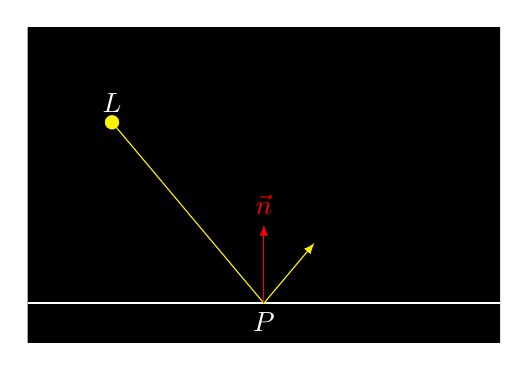
\begin{tikzpicture}
  \path[clip] (-3,-0.5) rectangle (3,3.5);
  \draw[fill=black,black] (-3,-1.5) rectangle (3,3.5);
  \draw[thick,white] (-3,0) -- (3,0);

  \coordinate (light) at (130:3);
  \coordinate (hit) at (0,0);
  
  \draw[fill=yellow] (light) circle [radius=0.1cm] node [white,above] {$L$};
  \node[anchor=north,white] at (hit) {$P$};

  \draw[yellow,-latex] (light) -- (hit) -- ++(50:1);
  \draw[red,-latex] (hit) -- ++(0,1) node[above] {$\vec n$};
\end{tikzpicture}

\end{document}